%---
\section{Project Overview}
\label{sec:ProjectOverview}

\begin{figure*}[t!]
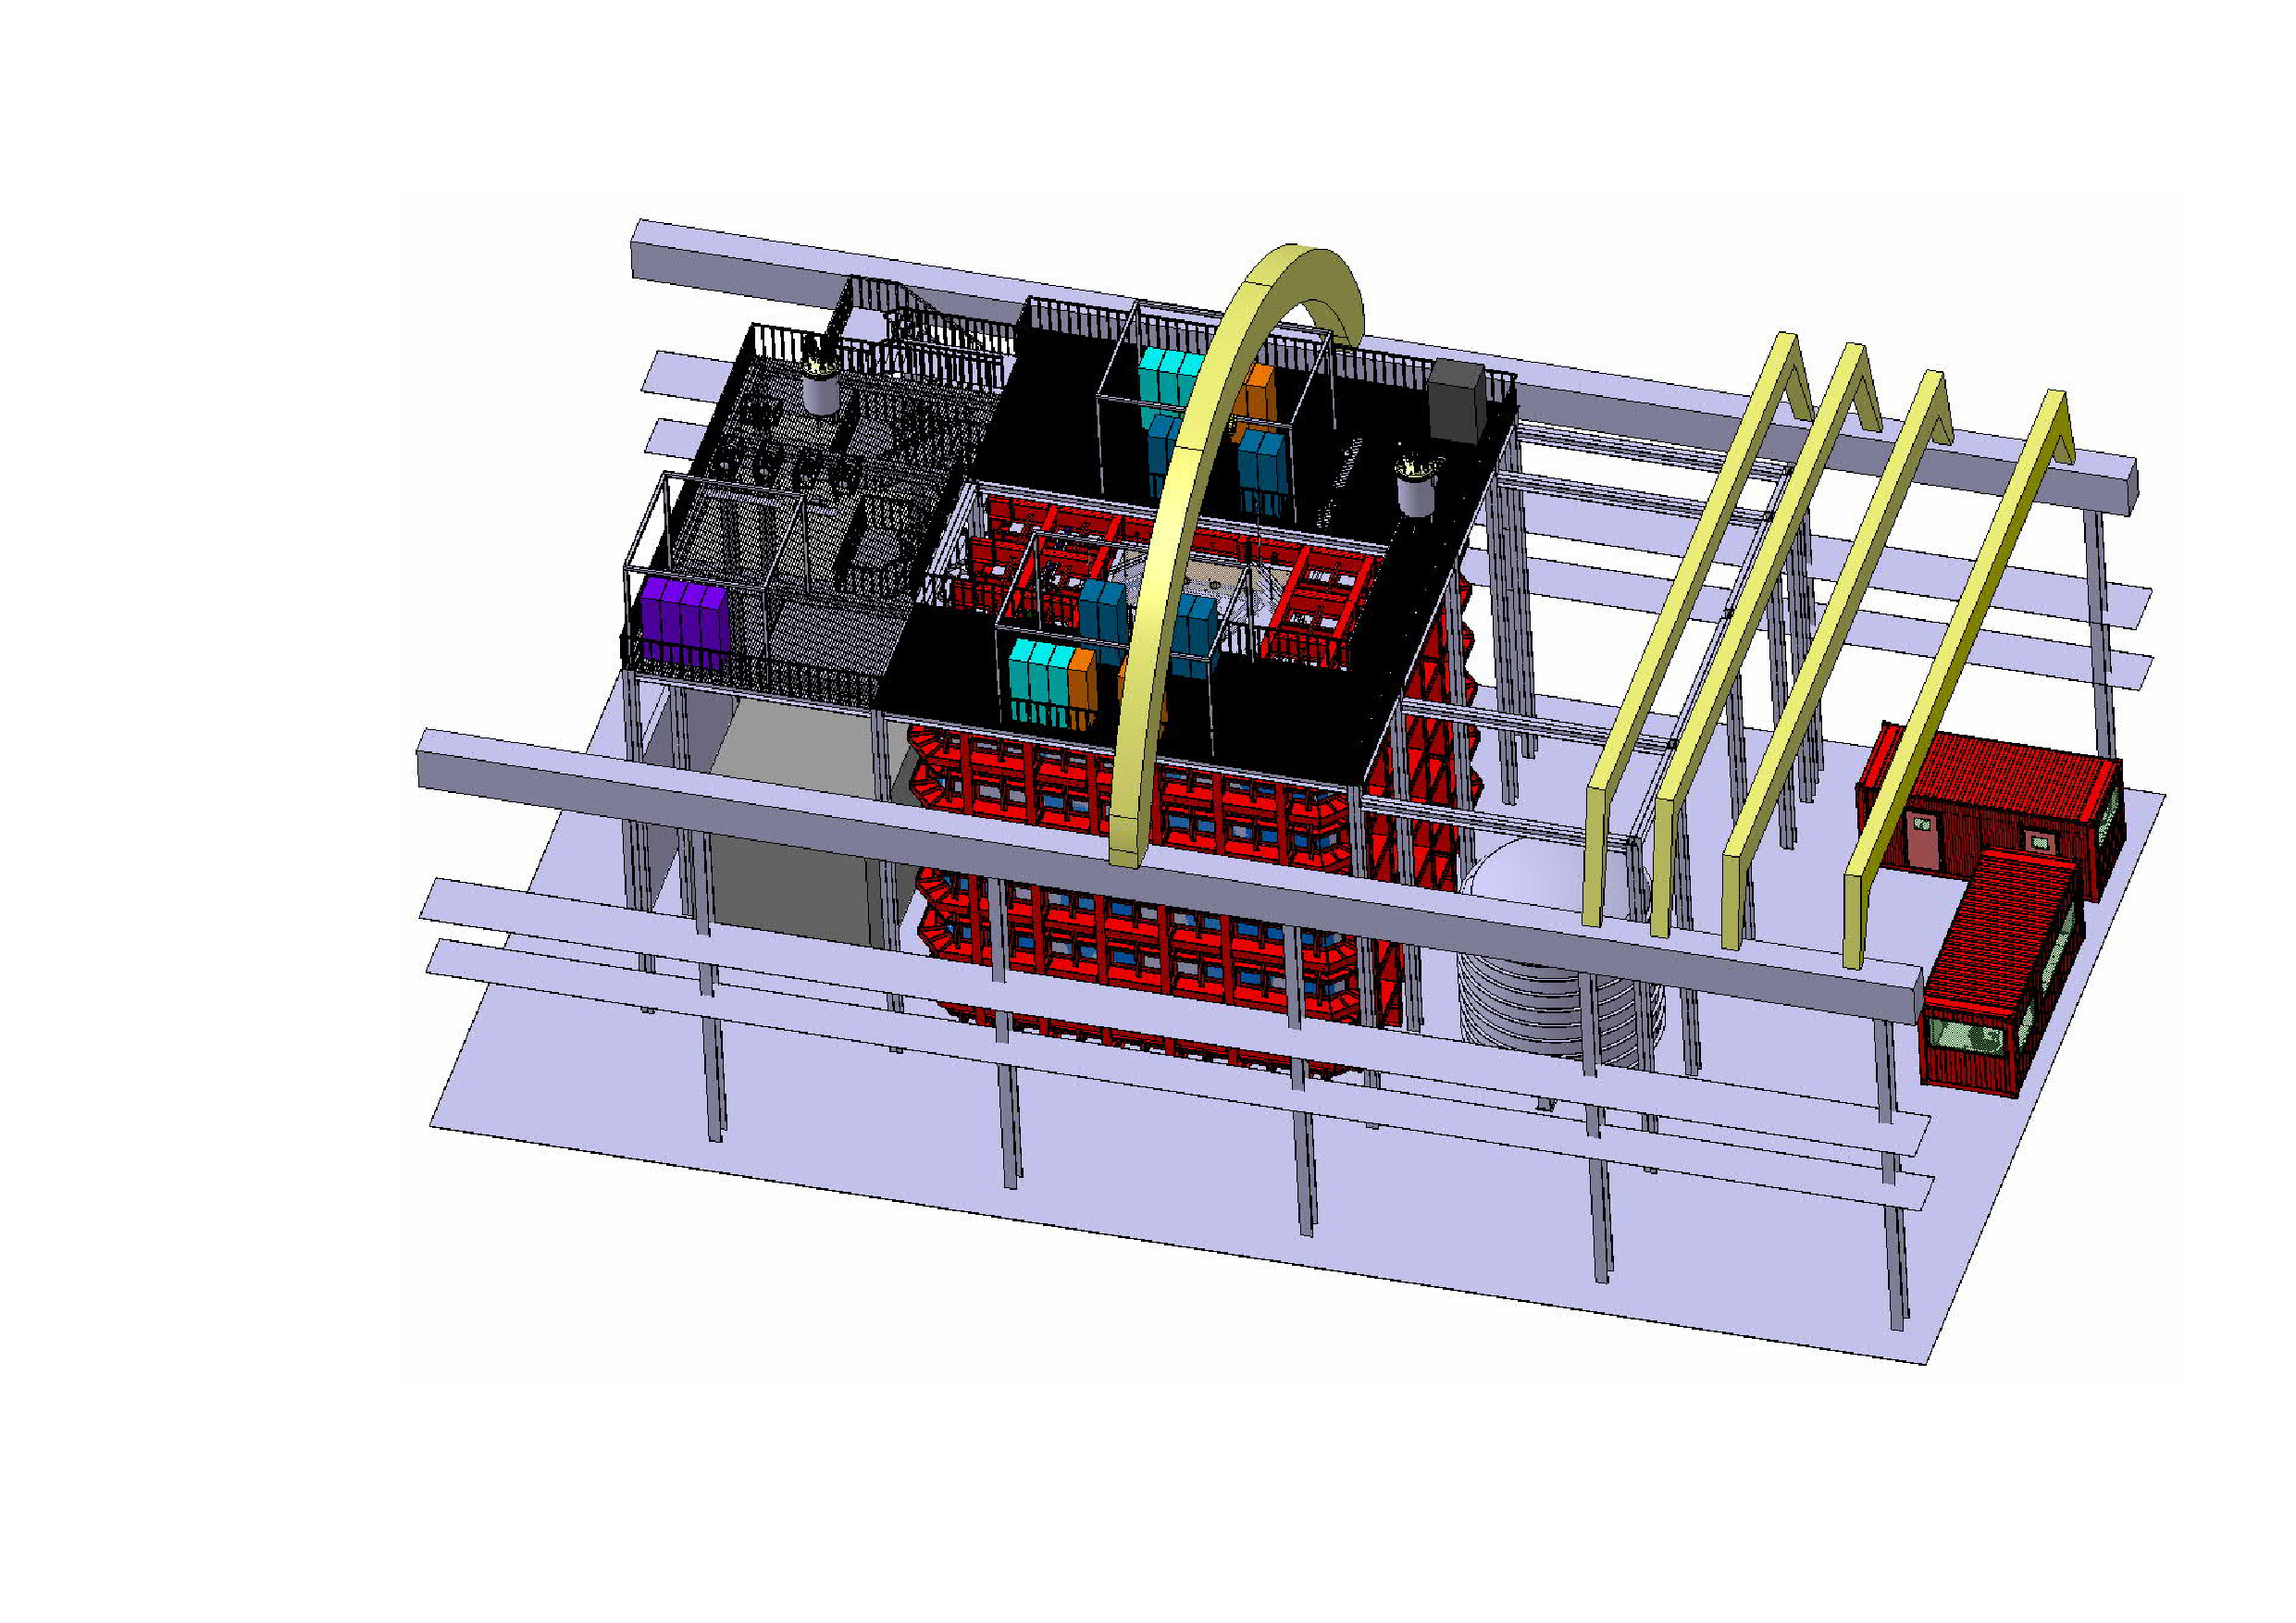
\includegraphics[width=\textwidth]{./Figures/DSk-Overall.pdf}
\caption[Artist rendering of the \DSks\ experiment in Hall C of \LNGS]{Artist rendering of the \DSks\ experiment in Hall C of \LNGS.}
\label{fig:Overall-Design}
\end{figure*}

Many fundamental design parameters for the \DSk\ (\DSks) experiment are based on the successful experience of the \DS\ Collaboration in constructing, commissioning, and operating the \DSf\ (\DSfs) detector in a background-free mode. The many technical details of \DSf\ can be found in~\cite{Agnes:2015gu,Agnes:2016cp,Agnes:2016fw,Agnes:2016fz,Agnes:2016tx,Agnes:2017ck,Agnes:2017cl,Agnes:2017cz,Agnes:2017ec,Agnes:2018cn,Agnes:2018dt,Agnes:2018ep,Agnes:2018fg,Agnes:2018ft}.  The \DSks\ liquid argon time projection chamber (\LArTPC) will, too, be deployed at \LNGS\ in the underground Hall\,C, at the center of a newly constructed active veto system.  \reffig{Overall-Design} shows the rendering of the future installation of \DSks\ in the underground Hall~C of \LNGS and \reffig{DSk3D} shows an overview of the detailed arrangement of the \LArTPC\ and its anti-coincidence veto detector.  The \DSks\ experiment is designed to operate for a minimum of \DSkExtendedRunTimePlanned\ while maintaining an irreducible background level in the \WIMP\ search region of less than \BackgroundFreeRequirement\ for the total exposure.  To achieve this goal, the design parameters of the \DSks\ experiment have been taken directly from \DSfs, where possible.  Design changes have been made where needed in order to accommodate for the much larger size of \DSks\ and to allow the experimental design to be scalable to a detector at the multi-hundred tonne scale.  In building this preliminary design, issues that have arisen because of design choices or materials selections have been dealt with by limited design modifications, and further optimization will continue as the final development work is completed and a full technical design is made.  

\DSks\ will be built by the Global Argon Dark Matter Collaboration (GADMC) and will consist of two detectors: the inner detector and the veto detector, both hosted in a \pDUNE-like cryostat~\cite{Abi:2017wp,Acciarri:2016wz}.   The inner detector is a \LArTPC\ filled with underground argon (\UAr).  The veto detector is made of a plastic shell, loaded with Gd, surrounding the inner detector, sandwiched between two active atmospheric argon (\AAr) layers.  

\begin{figure}[t!]
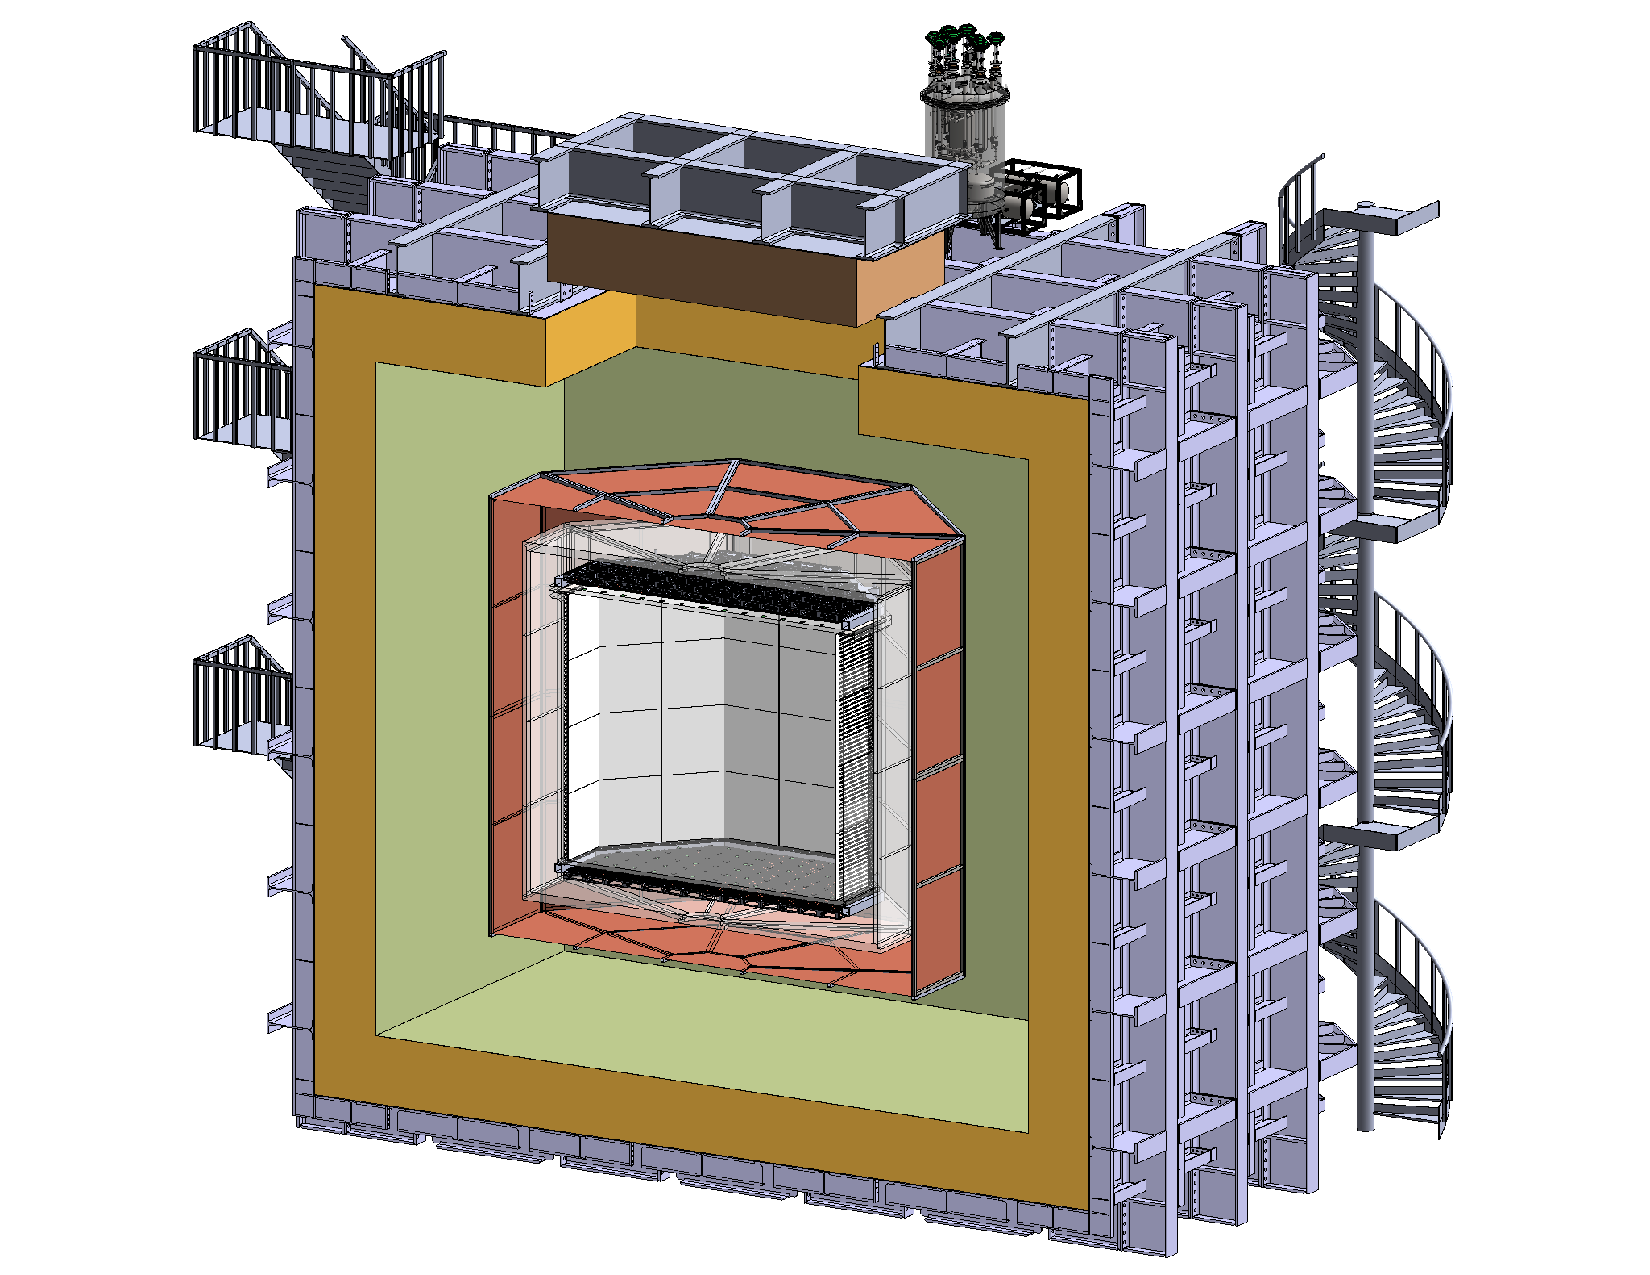
\includegraphics[width=\columnwidth]{Figures/DSk3D.pdf}
\caption[Artist rendering of the \DSks\ detectors]{Artist rendering of the \DSks\ detectors, with many components omitted for clarity of presentation.  The drawing shows the acrylic (\PMMA) sealed \TPC\  filled with \UAr, surrounded by the veto detector consisting of a \ce{Gd}-loaded acrylic Shell (\GdAS) sandwiched between two atmospheric argon (\AAr) active layers (the Inner Active Buffer, \IAB\ and the Outer Active Buffer, \OAB), all contained in the \pDUNE-like cryostat.  The \OAB\ is optically separated from the rest of the  \AAr\ by a copper vessel.  Technical designs of the support structure of the \TPC\ are already available, and intentionally omitted for clarity of presentation of the main elements.}
\label{fig:DSk3D}
\end{figure}

The decision to abandon an organic liquid scintillator veto and to host \DSks\ within a \pDUNE-like cryostat was originally motivated by the need of minimizing the environmental impact on underground \LNGS\ operations, but carries significant performance advantages.  Indeed, operating the \TPC\ directly in the \pDUNE-like cryostat eliminates the need of a cryostat in the immediate proximity of the \UAr\ target, which would significantly contribute to the residual background.  We therefore adopted a new design, with the \UAr-filled \TPC\  immersed in a bath of liquefied \AAr\ held at the same temperature and pressure.  This then allows for the use of a \TPC\ vessel fabricated from the same ultra-pure poly(methyl methacrylate) (acrylic or \PMMA) developed for the \DEAP\ experiment, and thus eliminating the need for a dedicated cryostat or \UAr\ containment vessel.  The outer walls of the \TPC\ will sit approximately \SI{2}{\m} away from inner wall of the cryostat.  The \pDUNE-like cryostat may be surrounded by layers of plastic for moderation of cosmogenic and radiogenic neutrons from the rocks surrounding the \LNGS\ Hall\,C, this option is being investigated.

While this overview section gives a general outline of the project and introduces the major features of the experiment as they stand in the current preliminary design, the real details are given in the subsequent sections. The development of the \SiPM\ photosensors, the \LArTPC\ and its cryogenics and gas handling system, and the materials screening plan that will ensure the radio purity of the experiment, are detailed in Sec.~\ref{sec:PE}, Sec.~\ref{sec:TPCCryo} and Sec.~\ref{sec:Materials}, respectively.  The plan for the calibration of the experiment is given in Sec.~\ref{sec:Calibration}, the design of the veto detector is presented in Sec.~\ref{sec:Veto}, and the details about the data acquisition system and the plan for offline computing are given in Sec.~\ref{sec:DAQ} and Sec.~\ref{sec:Computing}, respectively.  The two ancillary detectors, ReD and \DSp, are described in Sec.~\ref{sec:Red} and Sec.~\ref{sec:Proto}.  Finally, the design and use of the atmospheric argon cryostat, modeled after the ones deployed for ProtoDUNE, are given in Sec.~\ref{sec:Cryostat}, while the procurement of the underground argon (\UAr) target is detailed in the final section, Sec.~\ref{sec:Argon}.  Note that the following forms a preliminary design for an experiment capable of the stated physics goals, but may change as the technical details evolve in the final engineering stages.  \DSks\ will be built to operate for a minimum of \DSkExtendedRunTimePlanned, providing the best sensitivity to high-mass \WIMP\ dark matter.

Energy deposits in the \LAr\ target result in the production of excited and ionized argon atoms, according to the underlying process for recoiling electrons or nuclei. Excited argon atoms, which can also be produced by recombining ionization charge, lead to an efficient formation of argon excimers decaying via the emission of scintillation light characterized by two decay time constants. Both of the components are combine to yield an instant light signal, called \SOne. Due to the deep UV nature (around \ArWaveLength) of this scintillation light, which is absorbed by most materials, a thin layer of wavelength shifter, tetraphenyl butadiene (TPB), must cover all exposed surfaces to convert the photons to those of optical wavelengths for detection by photosensors. Ionization electrons escaping recombination are drifted to the top of the \LAr\ by an applied electric field, where an electric field stronger than the field applied to drift the electrons, extracts the electrons into the gas pocket above the liquid. Here the strong field accelerates the electrons, enough for them to excite (but not ionize) the argon gas, producing a secondary scintillation signal \STwo, proportional to the ionization charge.  Photosensors placed behind the wavelength shifter-coated windows at the top and bottom of the \TPC, read out both scintillation signals (\SOne\ and \STwo) of each event. \SOne\ is used for energy determination, as well as for pulse shape discrimination (PSD).  The latter is derived from the ratio of the prompt and delayed light fractions. \STwo\ is used for energy and 3D position measurements of the event, the vertical coordinate is measured from the drift time between \SOne\ and \STwo, and the horizontal coordinates from the light pattern resulting in the top photosensors from \STwo. 

The octagonal \LArTPC\ will have a height of \DSkActiveHeight\ and a distance between parallel walls of \DSkActiveDiameter.  It will be instrumented with a new kind of photosensors, arrays of \SiPMs, arranged in assemblies called photodetector modules (\DSkPdms). Each \DSkPdm\ has an area comparable to that of a \SI{3}{\inch} photomultiplier tube (\PMT ), with the \LArTPC\ containing \DSkTilesNumber\ \DSkPdms\ in total.  Substantial effort was put into the development of this technology, since \SiPMs\ promise a higher effective quantum efficiency, higher reliability at \LAr\ temperature, and a much higher radiopurity than \PMTs. All of these properties are crucial for \DSks\ since the PSD, which is the most important mechanism for background discrimination in \LAr, depends critically on the light yield.  Additionally, the large material budget of \PMTs\ is often a limiting factor for neutron- and gamma-induced backgrounds. The \LArTPC\ will be equipped with arrays of \SiPMs, totaling \DSkTilesArea\ in area.

In comparison to \DSfs, where a full digitization and recording of the waveform of each \PMT\ could be achieved, a custom scheme for the sampling of the two-orders-of-magnitude higher channel count of the \DSks\ \SiPM\ \DSkPdms\ has to be developed. Design parameters for the data acquisition (DAQ) system are driven by rates and occupancies, as well as leading edge timing and limited charge information from each channel, while compromising as little as possible on energy resolution and pulse-shape discrimination. %The DAQ system is described in Sec.~\ref{sec:DAQ}.

All components of the detector, especially the inner components, like the \LArTPC, the \SiPM\ arrays, and cables, must be made from materials of the highest radiopurity to keep backgrounds as small as possible.

The veto detector consists of three separate volumes:

\begin{compactitem}
\item An inner volume of active liquid \AAr, called the Inner Argon Buffer (\IAB), surrounding the \TPC;
\item A passive shell of acrylic loaded with Gd, called the \ce{Gd}-loaded Acrylic Shell (\GdAS), of octagonal shape mounted around the \IAB.  The \GdAS\ surrounds the TPC in all directions (lateral, top and bottom, with exceptions due to the signal and utility service holes). 
\item An outer active volume of \AAr, called the Outer Argon Buffer (\OAB).
\end{compactitem}

A copper cage which acts as a Faraday cage provides the optical insulation from the rest of the \AAr\ external to OAB and, at the same time, it realizes the necessary electric shield for reducing external noise from contaminating the detector signals.  The details of the veto design and expected performance are given in Sec.~\ref{sec:Veto}.

In order to demonstrate and test technological developments on a scale relevant to \DSks, the collaboration will build and operate a \DSpApproximateMass\ prototype. The project is called \DSp\ (\DSps) and is described in Sec.~\ref{sec:Proto}. \DSp\ will be at an intermediate scale between \DSfs\ and \DSks, able to test a number of full size components intended for use in \DSks.  The size of \DSps\ was chosen to be able to validate detector and \DSkPdm\ components, including the readout system, both from the mechanical and performance aspects of the experiment. The full size cryogenic system will also be tested in this way, especially the argon condenser, the gas pump, and the heat recovery system. Functionality and stability control, as well as safety issues during power failures, purification flow rates and general controls are meant to be explored. \DSps\ also serves to validate the readiness of the various production lines in the different institutions of the collaboration to ensure quality control and assurance for the production of components for \DSks.


%---
%\subsection{Calibrations}
%\label{sec:Overview-Calibrations}

For the \DSk\ detector to reach its physics goals, a comprehensive plan of calibrations for the \LArTPC\ and Veto detectors is necessary.  The calibration equipment and techniques specific to the \DSks\ experiment are described in detail in Sec.~\ref{sec:Calibration}.  In addition to this, it will be important to also utilize measurements taken with external calibration experiments placed within the line of sight of a neutron beam.  In the \SCENE\ experiment,\cite{Cao:2015ks,Alexander:2013ke} a monochromatic, low energy, pulsed neutron beam at the Notre Dame Institute for Structure and Nuclear Astrophysics was used to study the scintillation light yield from recoiling nuclei in a small \LArTPC, but only down to \SCENERecoilsEnergyMax.  The \ARIS\ experiment was exposed to the highly collimated and quasimonoenergetic LICORNE neutron beam at the Institut de Physique Nucl\'eaire d'Orsay (IPNO) in order to study the scintillation response to nuclear and electronic recoils~\cite{Agnes:2018cn}.

The collaboration is now expanding this external calibration work with a new external calibration experiment, the Recoil Directionality (\ReD ) experiment, described in Sec.~\ref{sec:Red}. The \ReD\ detector is a small \LArTPC\ (similar in size to \SCENE ) equipped with the same \SiPM\ tiles planned for use in \DSks. \ReD\ is designed to select and measure single neutron elastic scatters on argon nuclei, by means of a large acceptance neutron spectrometer, composed of an array of liquid scintillator detectors.  Kinematic requirements of the neutron interactions will allow for the precise detection of nuclear recoils in the \LAr, since the neutron energy, scattering angle, and drift field direction can all be precisely measured with the use of external neutron detectors.

